\documentclass[11pt,a4paper]{article}
\usepackage[utf8]{inputenc}
\usepackage{amsmath}
\usepackage{amsfonts}
\usepackage{amssymb}
\usepackage{array}
\usepackage{latexsym}
\usepackage{textcomp}
\usepackage{graphicx}
\usepackage{fullpage}
\usepackage{float} 

\author{Erich L. Foster - Robin Goix}
\title{Optimal shape design of wave makers}

\begin{document}
	\maketitle

	\tableofcontents
	\addcontentsline{toc}{section}{Introduction}
	
	\pagebreak
	
	\section*{Introduction}
	The aim of this report is to provide a mathematical and computational framework for the problem of water wave generation. Our interest is in modelling the generation of wave by an underwater moving object, to develop a computational framework for this problem and then to use it in order to optimize the shape and trajectory of the underwater moving object.
		
		\pagebreak
		
	\section{Physical modelling of waves}
		The first step is to find an appropriate model to represent our problem. We aim at modelling the creation and propagation of breaking waves to surf, which occurs near the shore where the seabed rises. We will therefore make some assumptions so as to find an accurate model as simple as possible. We will consider water as an incompressible and inviscid fluid.
		
		\subsection{Shallow water equations}
			The first model we shall consider are the shallow water equations, or Saint Venant equations). Starting from 
the Euler equations and the kinematic and dynamic boundary conditions:
			\begin{align}
				\displaystyle (\frac{\partial}{\partial t} + \mathbf{u} \cdot \mathbf{\nabla}) \; \mathbf{u} & = \displaystyle -\frac{1}{\rho}\nabla p + \mathbf{g} \\
				\mathbf{\nabla} \cdot \mathbf{u} & = 0 
			\end{align}
			\begin{align}
				\frac{\mathrm{d}}{\mathrm{d} t} \eta(x,y,t) & = w(x,y \eta) \\
				p  = p_a & = 0 \: \: \:  \: \: \: \mathrm{for} \: z=\eta \\ 
				-\frac{\mathrm{d}}{\mathrm{d}t} h(x,y,t) & = w(x,y,h)
			\end{align}
			the following assumptions:
			\begin{itemize}
				\item The typical water depth $h_0$ is small compare to the horizontal scale $\lambda_0$, i.e. $\sigma = \frac{h_0}{\lambda_0} \ll 1 $;
				\item The horizontal velocity $\mathbf{u}_h = (u,v)$ is independent of z. We have therefore $\mathbf{u}_h =$
			\end{itemize}			
			 lead us to the following system, which are the Shallow water equation (or Saint-Venant equations)
			\begin{align}
				\mathbf{u}_t + \nabla\eta + \epsilon (\mathbf{u} \cdot \nabla) \mathbf{u} &= 0 \label{SWE1}\\
				\eta_t + \zeta_t + \nabla \cdot [(h+\epsilon \eta) \mathbf{u}] &= 0 \label{SWE2}
			\end{align}						
			The detail of the derivation for can be found in \cite{JMC2013}.
			\pagebreak
			
		\subsection{Peregrine System}
			(Cf. \cite{DM2013}).\\ 
			As illustrated in Figure \ref{Coordinates}, we consider $(\tilde{x},\tilde{y},\tilde{z})$ a Cartesian coordinate system, with $\tilde{z}$ measuring upwards from the still water level. We call $\tilde{\eta}(\tilde{x},\tilde{y},\tilde{t})$ the height of the free surface at a time $\tilde{t}$, and $\tilde{h}(\tilde{x},\tilde{y},\tilde{t}) = \tilde{D}(\tilde{x},\tilde{y}) + \tilde{\zeta}(\tilde{x},\tilde{y}, \tilde{t})$ the seabed profile, which is assumed to be the sum of a time-independent part $\tilde{D}$ - the seabed -, and a time-dependant part $\tilde{\zeta}$ - the underwater moving object.
			\begin{figure}[h]
				\centering
				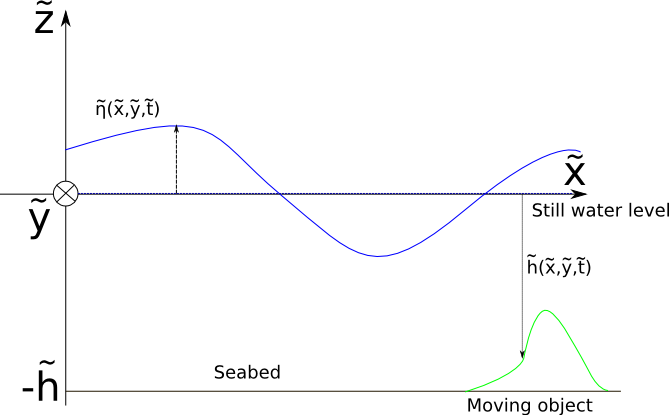
\includegraphics[height=6cm]{CartesianCoordinates.png}
				\caption{Reference}
				\label{Coordinates}
			\end{figure}
			
			Denoting $\mathbf{\hat{u}} = (\tilde{u},\tilde{v}, \tilde{w})$ the fluid velocity, $\hat{P}$ the pressure field, $\rho$ the density and $\mathbf{g} = (0,0,g)$ the gravity, the Euler equations are written: 
			\begin{align}
						\displaystyle \mathbf{\hat{u}}_{\tilde{t}} + (\mathbf{\hat{u}} \cdot \tilde{\nabla}) \mathbf{\hat{u}} + \frac{1}{\rho} \tilde{\nabla}\tilde{P} &=  -\mathbf{g} \label{Euler1} \\
						\tilde{\nabla} \cdot \mathbf{\hat{u}} & = 0 \\
						\tilde{\nabla} \times \mathbf{\hat{u}} & = 0 \label{Euler3}
			\end{align}
			The kinematic boundary condition at the free surface expresses the equality between the vertical velocity and the total derivative of $\tilde{\eta}$, whereas the kinematic boundary condition at the bottom expresses the equality between the vertical velocity and the total derivative of $\tilde{h}$:
			\begin{align}
				\frac{\mathrm{d}}{\mathrm{d}\tilde{t}} \tilde{\eta}(\tilde{x},\tilde{y},\tilde{t}) & = \tilde{w}(\tilde{x},\tilde{y},\tilde{\eta}) \label{BC1} \\
				-\frac{\mathrm{d}}{\mathrm{d}\tilde{t}} \tilde{h}(\tilde{x},\tilde{y},\tilde{t}) & = \tilde{w}(\tilde{x},\tilde{y},-\tilde{h}) \label{BC2}
			\end{align}
			At the free surface $\tilde{z} = \tilde{\eta}(\tilde{x},\tilde{y},\tilde{t})$,	the fluid is also assumed to satisfy the dynamic boundary condition $\tilde{P}(\tilde{x},\tilde{y},\tilde{t}) = \tilde{P}_0(\tilde{x},\tilde{y})$.
			
			Considering a characteristic water depth $h_0$ and the corresponding 	characteristic velocity $c_0 = \sqrt{g h_0}$, a typical wavelength $\lambda_0$ and a typical wave height $a_0$, we scale the variables as in \cite{DM2013}: 
			\begin{equation*}
				x = \frac{\tilde{x}}{\lambda_0},\: 
				y = \frac{\tilde{y}}{\lambda_0}, \:
				z = \frac{\tilde{z}}{h_0}, \: 
				t = \frac{c_0}{\lambda_0}\tilde{t}
			\end{equation*}
			\begin{equation*}
				u = \frac{h_0}{a_0 c_0} \tilde{u},\:
				v = \dfrac{h_0}{a_0 c_0} \tilde{v},\:
				w = \dfrac{\lambda_0}{a_0 c_0} \tilde{w},\: 
				\eta = \dfrac{\tilde{\eta}}{a_0},\: 
				h = \dfrac{\tilde{h}}{h_0},\:
				D = \dfrac{\tilde{D}}{h_0}, \:
				\zeta = \dfrac{\tilde{\zeta}}{a_0},\:
				P = \dfrac{\tilde{P}}{\rho c_0^2}				
			\end{equation*}
			We separate the vertical and horizontal velocity, such as $\mathbf{u} = (u,v)$ and $\nabla = (\partial_x,\partial_y)$, and we consider $\epsilon = a_0 / h_0$ and $\sigma = h_0 / \lambda_0$ to be small. The dimensionless form of the equations \eqref{Euler1} - \eqref{Euler3} are therefore given by: 
			\begin{align}
				\epsilon \mathbf{u}_t + \epsilon^2((\mathbf{u} \cdot \nabla) \mathbf{u} + w \mathbf{u}_z) + \nabla P & = 0 \label{MConsxy}\\
				\epsilon \sigma^2 w_t + \epsilon^2 \sigma^2 ((\mathbf{u} \cdot \nabla w) + w w_z) + P_z & = -1 \label{MConsz}\\
				\nabla \cdot \mathbf{u} + w_z & =  0 \label{MassCons}\\
				u_y-v_x & = 0 \label{Irrxy}\\
				\mathbf{u}_z - \sigma^2 \nabla w & = 0 \label{Irrz}
			\end{align}
			and the dimensionless form of the boundary conditions \eqref{BC1} - \eqref{BC2} are: 
			\begin{align}
				\eta_t + \epsilon (\mathbf{u} \cdot \nabla \eta ) & = w & \mathrm{on} \: z =\epsilon \eta \label{BCH}\\
				- \zeta_t - \mathbf{u} \cdot \nabla h & = w & \mathrm{on} \:  z = -h
				\label{BCB}
			\end{align}
			where $h = D + \epsilon \zeta $.
			
			Integrating equation \eqref{MassCons} with respect to $z$ from $-h$ to $z$, and using \eqref{BCB} we have: 
			\begin{equation}
				w = -\mathbf{u} \cdot \nabla h - \int^z_{-h} \nabla \cdot \mathbf{u} - \zeta_t 
				\label{Eq1}
			\end{equation}
			After integration of equation \eqref{Irrz} and using \eqref{Eq1}, we observe 
			\begin{equation}
				\mathbf{u} = \mathbf{u}_b + O(\sigma^2) \label{ApproxVelocity}
			\end{equation}
			where $\mathbf{u}_b$ is the horizontal velocity of the fluid at the bottom $z=-h$. Substitution of \eqref{Eq1} into the irrotationality condition \eqref{Irrz}, and using \eqref{ApproxVelocity}, yields:
			\begin{equation}
				\mathbf{u}_z = -\sigma^2\nabla(\nabla \cdot (h \mathbf{u}_b)) - \sigma^2 z \nabla(\nabla \cdot \mathbf{u}_b) - \sigma^2 \nabla \zeta_t + O(\sigma^4) 
				\label{Eq:u_z}
			\end{equation}
			Integration of \eqref{Eq:u_z} with respect to $z$ from $-h$ to $z$ gives
			\begin{equation}
				\mathbf{u} = \mathbf{u}_b - \sigma^2(z+h)\nabla (\nabla \cdot (h \mathbf{u}_b)) - \sigma^2 \frac{z^2-h^2}{2}\nabla ( \nabla \cdot \mathbf{u}_b) - \sigma^2(z+h)\nabla \zeta_t + O(\sigma^4) \label{ApproxVelocity2}
			\end{equation}
			We note than \eqref{ApproxVelocity} and \eqref{Eq1} lead to: 
			\begin{equation}
				w = - \nabla \cdot (h \mathbf{u}_b) - z \nabla \cdot \mathbf{u}_b - \zeta_t + O(\sigma^2)
			\end{equation}
			and then:
			\begin{equation}
				w_t = - \nabla \cdot (h \mathbf{u}_b)_t - z \nabla \cdot (\mathbf{u}_b)_t - \zeta_{tt} + O(\sigma^2) \label{Eq:2} 
			\end{equation}
			Assuming that $P = 0$ at $z = \epsilon\eta$, integrating \eqref{MConsz} with respect to $z$ from $z$ to $\epsilon\eta$, and using \eqref{Eq:2} we obtain
			\begin{equation}
				P = \epsilon \sigma^2(z\nabla \cdot (h \mathbf{u}_b)_t + \frac{z^2}{2} \nabla \cdot (\mathbf{u}_b)_t) + \epsilon \sigma^2z \zeta_{tt} + \epsilon \eta - z + O(\epsilon\sigma^4, \epsilon^2 \sigma^2)
			\end{equation}
			Using equations \eqref{MConsxy} and \eqref{ApproxVelocity2}, for $z = -h$, and considering the fact that $h_t = O(\epsilon)$, we have
			\begin{equation}
				(\mathbf{u}_b)_t + \nabla \eta + \epsilon (\mathbf{u}_b \cdot \nabla)\mathbf{u}_b - \sigma^2 h \nabla (\nabla \cdot (h (\mathbf{u}_b)_t)) + \sigma^2 \frac{h^2}{2} \nabla (\nabla \cdot (\mathbf{u}_b)_t) - \sigma^2 h \nabla \zeta_{tt} = O(\sigma^4, \epsilon \sigma ^2) \label{Eq:3}
			\end{equation}
			Integration of the conservation of mass \eqref{MassCons} with respect to $z$ from $-h$ to $\epsilon\eta$ yields
			\begin{equation}
				w(\epsilon\eta) - w(-h) = - \int^{\epsilon\eta}_{-h} \! \nabla \cdot \mathbf{u} \; \mathrm{dz}
			\end{equation}
			and thus, adding the boundary conditions \eqref{BCB} and \eqref{BCH} we have
			\begin{equation}
				\eta_t + \nabla \cdot \int^{\epsilon\eta}_{-h}\ \mathbf{u} \; \mathrm{dz} 
				\label{BoundaryEq}
			\end{equation}
			
			Denote the depth-average horizontal velocity of the fluid by 
			\begin{equation}
				\bar{\mathbf{u}} = \frac{1}{h+\epsilon \eta} \int^{\epsilon\eta}_{-h}\! \mathbf{u} \; \mathrm{dz} \label{AverageVelocity}
			\end{equation}
			then \eqref{BoundaryEq} becomes 
			\begin{equation}
				\eta_t + \zeta_t + \nabla \cdot [(h + \epsilon \zeta) \bar{\mathbf{u}}] = 0 
				\label{Eq:Sys2}
			\end{equation}
			Using the depth-average velocity \eqref{AverageVelocity} in
			\eqref{ApproxVelocity2} we obtain: 
			\begin{equation}
				\mathbf{u}_b = \bar{\mathbf{u}} + \sigma^2\frac{h}{2} \nabla (\nabla \cdot (h \bar{\mathbf{u}}) - \sigma^2 \frac{h^2}{3} \nabla (\nabla \cdot \bar{\mathbf{u}}) + \sigma^2 \frac{h}{2} \nabla \zeta_t + O(\sigma^4, \epsilon \sigma^2) 
			\end{equation}
			and thus, the equation \eqref{Eq:3} gives: 
			\begin{equation}
				\bar{\mathbf{u}}_t + \nabla \eta + \epsilon(\bar{\mathbf{u}} \cdot \nabla) \bar{\mathbf{u}} - \sigma^2 \frac{h}{2} \nabla ( \nabla \cdot (h\bar{\mathbf{u}}_t)) + \sigma^2 \frac{h^2}{6}\nabla ( \nabla \cdot \bar{\mathbf{u}}_t) - \sigma^2\frac{h}{2}\nabla \zeta_{tt} = O(\epsilon \sigma^2, \sigma^4) \label{Eq:Sys1}
			\end{equation}
			
			To reduce the amount of notation, the depth-average velocity will subsequently be denoted $\mathbf{u}$. With equations \eqref{Eq:Sys1} and \eqref{Eq:Sys2}, we obtain the Boussinesq system of equations similar to \cite{Peregrine}.
			\begin{center}
				$\left\lbrace
					\begin{array}{rll}
						\displaystyle \mathbf{u}_t + \nabla \eta + \epsilon (\mathbf{u} \cdot \nabla)\mathbf{u} - \sigma^2\frac{h}{2}\nabla (\nabla \cdot (h \mathbf{u}_t)) + \sigma^2 \frac{h^2}{6}\nabla (\nabla \cdot \mathbf{u}_t) - \sigma^2\frac{h}{2}\nabla \zeta_{tt}  & = & \displaystyle O(\epsilon \sigma^2, \sigma^4) \\
						\displaystyle \eta_t+\zeta_t + \nabla \cdot [(h+\epsilon\eta)\mathbf{u}] & = & 0
					\end{array}
				\right.$
			\end{center}
			
			\pagebreak
			
	\subsection{Equations in the moving object's referential}
	The aim of this section is to derive the systems introduced in the previous section into the referential of the moving object, assuming that it moves at constant velocity $\tilde{\mathbf{U}}_o = (\tilde{U}_{ox},\tilde{U}_{oy})$. The physical change of	variable would therefore be:
	\begin{equation*}
		\tilde{X} = \tilde{x} - \tilde{U}_{ox} \tilde t, \:
		\tilde{Y} = \tilde{y} - \tilde{U}_{oy} \tilde{t}, \:
		\tilde{Z} = \tilde{z}, \:
		\tilde{T} = \tilde{t}	
	\end{equation*}
	Scaling the variables as described in the previous section and using the dimensionless variables:
	\begin{equation*}
		X = \frac{\tilde{X}}{\lambda_0}, \;
		Y = \frac{\tilde{Y}}{\lambda_0}, \;
		Z = \frac{\tilde{Z}}{h_0}, \;
		\mathbf{U}_o = \frac{h_0}{a_0 c_0} \tilde{\mathbf{U}_o}
	\end{equation*}
	the change of variables for our dimensionless systems is therefore: 
	\begin{equation*}
		X = x - \epsilon U_{ox} t, \:
		Y = y - \epsilon U_{oy} t, \:
		Z = z, \:
		T = t	
	\end{equation*}
	And we have:
	\begin{equation}
		\partial_x = \partial_X, \;
		\partial_y = \partial_Y, \;
		\partial_z = \partial_Z, \;
		\partial_t = \partial_T - \epsilon \mathbf{U}_o \cdot \nabla \label{ChangeOfReferential}
	\end{equation}
	
		\subsubsection{Shallow water equations}
		Assumption: 
		\begin{itemize}
			\item Constant object's velocity $\mathbf{U}_o$
			\item $D_T = 0$ (the seabed does not change in the object's motion direction)
		\end{itemize}
		Starting from the equations \eqref{SWE1} and \eqref{SWE2} and using \eqref{ChangeOfReferential} and the fact that $h_t = \epsilon \zeta_t$, we obtain:
		\begin{align}
			\eta_T + \nabla \cdot [(\epsilon \eta + h)(\mathbf{u} - \mathbf{U}_o)] &= 0 \\
			\mathbf{u}_T + \nabla \eta		+ \epsilon ((\mathbf{u} - \mathbf{U}_o)\cdot \nabla) \mathbf{u} &= 0
		\end{align}
		With $\mathbf{u_\Delta} = \mathbf{u} - \mathbf{U}_o$, the system becomes:
		\begin{align}
			\eta_T + \nabla \cdot [(\epsilon \eta + h)\mathbf{u_\Delta}] &= 0 \\
			(\mathbf{u_\Delta})_T + \nabla \eta		+ \epsilon (\mathbf{u_\Delta}\cdot \nabla) \mathbf{u_\Delta} &= 0
		\end{align}
		
		
		\pagebreak
		
		\subsubsection{Peregrine system}
			Starting from the equations \eqref{SWE1} and \eqref{SWE2} and using \eqref{ChangeOfReferential} and the fact that $h_t = \epsilon \zeta_t$, we obtain:
			\begin{align}
				\mathbf{u}_T + \nabla \eta		+ \epsilon ((\mathbf{u} - \mathbf{U}_o)\cdot \nabla) \mathbf{u}  - \sigma^2\frac{h}{2}\nabla (\nabla \cdot (h \mathbf{u}_T)) + \sigma^2 \frac{h^2}{6}\nabla (\nabla \cdot \mathbf{u}_T) &= O(\epsilon \sigma^2, \sigma^4)\\
				\eta_T + \nabla \cdot [(\epsilon \eta + h)(\mathbf{u} - \mathbf{U}_o)] &= 0
	\end{align}
	
		With $\mathbf{u_\Delta} = \mathbf{u} - \mathbf{U}_o$, the system becomes:
		\begin{align}
			(\mathbf{u_\Delta})_T + \nabla \eta		+ \epsilon (\mathbf{u_\Delta}\cdot \nabla) \mathbf{u_\Delta} - \sigma^2\frac{h}{2}\nabla (\nabla \cdot (h \mathbf{u_\Delta}_T)) + \sigma^2 \frac{h^2}{6}\nabla (\nabla \cdot \mathbf{u_\Delta}_T) &= O(\epsilon \sigma^2, \sigma^4)\\
			\eta_T + \nabla \cdot [(\epsilon \eta + h)\mathbf{u_\Delta}] &= 0
		\end{align}			
			
		\pagebreak
	\section{Numerical solver for the Peregrine system}	
		\subsection{Weak Formulation of the Peregrine system}
	Denoting $\mathbf{u}$ the depth-average velocity, $h(x,y,t) = D(x,y) + \epsilon \zeta(x,y,t)$ the bottom, where  $D(x,y)$ is the natural profile of the bottom, whereas $\zeta$ characterize the shape of the moving underwater object. We look for the corresponding variational formulation of the following system: 
	\begin{align}
		\mathbf{u}_t + \nabla \eta + \epsilon (\mathbf{u} \cdot \nabla)\mathbf{u} - \sigma^2\frac{h}{2}\nabla (\nabla \cdot (h \mathbf{u}_t)) + \sigma^2 \frac{h^2}{6}\nabla (\nabla \cdot \mathbf{u}_t) - \sigma^2\frac{h}{2}\nabla \zeta_{tt}  &= O(\epsilon \sigma^2, \sigma^4) \label{Peregrine1}\\
		\eta_t+\zeta_t + \nabla \cdot [(h+\epsilon\eta)\mathbf{u}] &= 0 \label{Peregrine2}
	\end{align}
		
		Considering the fluid to be in a pool, we impose slip boundary conditions for the velocity on $\partial \Omega$, and introduce the space $\mathbb{V} = \left\lbrace \mathbf{w} \in \mathbb{H}^1(\Omega)^2, \mathbf{w} \cdot \mathbf{n} = 0 \: \mathrm{on} \: \partial \Omega \right\rbrace $, where $\mathbf{n}$ represent the normal to the boundary. Let $(\mathbf{v},\xi) \in \mathbb{V} \times \mathbb{H}^1(\Omega)$, then multiplying \eqref{Peregrine1} by $\mathbf{v}$ and \eqref{Peregrine2} by $\xi$ and integrating over the domain $\Omega$, we obtain:   
		\begin{equation}
			\begin{split}
				\int_{\Omega} \! \mathbf{u}_t \cdot \mathbf{v} \: \mathrm{dx} + \int_{\Omega} \! \nabla \eta \cdot \mathbf{v} \: \mathrm{dx} + \epsilon \! \int_{\Omega} \! (\mathbf{u} \cdot \nabla ) \mathbf{u} \cdot \mathbf{v} \: \mathrm{dx} - \sigma^2 \! \int_{\Omega} \! \frac{h}{2} \nabla (\nabla \cdot (h \mathbf{u}_t)) \cdot \mathbf{v} \: \mathrm{dx} \\
				+ \sigma^2 \! \int_{\Omega} \! \frac{h^2}{6} \nabla (\nabla \cdot \mathbf{u}_t) \cdot \mathbf{v} \: \mathrm{dx} - \sigma^2 \! \int_{\Omega} \! \frac{h}{2} \nabla \zeta_{tt} \cdot \mathbf{v} \: \mathrm{dx} = 0\\
				\int_{\Omega}\! \eta_t \; \xi \: \mathrm{dx} +\int_{\Omega}\! \zeta_t \; \xi \: \mathrm{dx} +\int_{\Omega}\! \nabla \cdot [(h+\epsilon\eta) \mathbf{u}] \; \xi \: \mathrm{dx} = 0
			\end{split}
			\label{PeregrineWeakForm1}
		\end{equation}
		Using divergence theorem and the fact that $\mathbf{v} \cdot \mathbf{n}$ and $\mathbf{u} \cdot \mathbf{n}$ vanish on the boundaries, we get: 
		\begin{equation}
			\begin{split}
				0 &= \int_{\Omega} \! \mathbf{u}_t \cdot \mathbf{v} \: \mathrm{dx} - \int_{\Omega} \! \eta \; (\nabla \cdot \mathbf{v}) \: \mathrm{dx} + \epsilon \! \int_{\Omega} \! (\mathbf{u} \cdot \nabla ) \mathbf{u} \cdot \mathbf{v} \: \mathrm{dx} + \frac{\sigma^2}{2} \! \int_{\Omega} \!  (\nabla \cdot (h \mathbf{u}_t)) \; (\nabla \cdot (h \mathbf{v}) )\: \mathrm{dx} \\
				&\quad - \frac{\sigma^2}{6} \! \int_{\Omega} \! (\nabla \cdot \mathbf{u}_t) \; (\nabla  \cdot (h^2  \mathbf{v})) \: \mathrm{dx} + \frac{\sigma^2}{2} \! \int_{\Omega} \!  \zeta_{tt}  \; (\nabla \cdot( h \mathbf{v})) \: \mathrm{dx}\\
				0 &= \int_{\Omega}\! \eta_t \; \xi \: \mathrm{dx} +\int_{\Omega}\! \zeta_t \; \xi \: \mathrm{dx} -\int_{\Omega}\! \nabla \xi \; \cdot [(h+\epsilon\eta) \mathbf{u}]  \: \mathrm{dx}
			\end{split} 
		\end{equation}
		Noticing that $\dfrac{\partial h}{\partial t} = \epsilon \dfrac{\partial 
		\zeta}{\partial t}$, we finally obtain: 
		\begin{equation}
			\begin{split}
				0 &= \int_{\Omega} \! \mathbf{u}_t \cdot \mathbf{v} \: \mathrm{dx} - \int_{\Omega} \! \eta \; (\nabla \cdot \mathbf{v}) \: \mathrm{dx} + \epsilon \! \int_{\Omega} \! (\mathbf{u} \cdot \nabla ) \mathbf{u} \cdot \mathbf{v} \: \mathrm{dx} + \frac{\sigma^2}{2} \! \int_{\Omega} \!  (\nabla \cdot (h 
\mathbf{u}_t)) \; (\nabla \cdot (h \mathbf{v}) )\: \mathrm{dx} \\ 
				&\quad - \frac{\sigma^2}{6} \! \int_{\Omega} \! (\nabla \cdot \mathbf{u}_t) \; (\nabla  \cdot (h^2  \mathbf{v})) \: \mathrm{dx} + \frac{\sigma^2}{2 \epsilon} \! \int_{\Omega} \!  h_{tt}  \; (\nabla \cdot( h \mathbf{v})) \: \mathrm{dx}\\
				0 &= \int_{\Omega}\! \eta_t \; \xi \: \mathrm{dx} +\frac{1}{\epsilon}\int_{\Omega}\! h_t \; \xi \: \mathrm{dx} -\int_{\Omega}\! \nabla \xi \; \cdot [(h+\epsilon\eta) \mathbf{u}]  \: \mathrm{dx}
			\end{split}
		\end{equation}
		
		\pagebreak
			\subsection{Weak Formulation with inhomogeneous boundary conditions}

				The main inconvenient of the previous model is that, as the object is moving along the mesh, we need to compute the simulation on a really large domain if we want to model the wave for a long time. A solution to that problem is to consider the object as a static object in a stream of velocity $\mathbf{\tilde U} = \tilde{U} \: \mathbf{e_x} $. In that framework, the previous Peregrine system still apply but the weak formulation is slightly different as the boundary conditions have changed.\\
				
				With $\mathbf{U} = \frac{h_0}{a_0 c_0} \mathbf{\tilde{U}}$, we introduce  $\mathbb{V}' = \left\lbrace \mathbf{w} \in \mathbb{H}^1(\Omega)^2, \mathbf{w} \cdot \mathbf{n} = 0 \: \mathrm{on} \: \partial \Omega_y, \mathbf{w} = \mathbf{0} \: \mathrm{on} \: \partial \Omega_x\right\rbrace $ and $\mathbb{U}' = \left\lbrace \mathbf{w} \in \mathbb{H}^1(\Omega)^2, \mathbf{w} \cdot \mathbf{n} = 0 \: \mathrm{on} \: \partial \Omega_y, \mathbf{w} = -\mathbf{U} \: \mathrm{on} \: \partial \Omega_x\right\rbrace $. As we still have $\mathbf{v} \cdot \mathbf{n} = 0 \: \forall \: \mathbf{v} \in \mathbb{V}'$, the boundary terms resulting from the divergence theorem apply to the last terms of the first equation of \eqref{PeregrineWeakForm1} are still null, but this is not the case for the second equation where we have: 
				\begin{equation}
					\int_{\Omega}\! \nabla \cdot [(h+\epsilon\eta) \mathbf{u}] \; \xi \: \mathrm{dx} = - \int_{\Omega}\! \nabla \xi \; \cdot [(h+\epsilon\eta) \mathbf{u}]  \: \mathrm{dx} + \int_{\partial \Omega_x} \! \xi (h+\epsilon \eta) \mathbf{u} \cdot \mathbf{n} \; \mathrm{ds}
				\end{equation}				
			
			\pagebreak
		\subsection{Discretization and FEM}	
		Let $\mathrm{dt}$ be a small time-step, the second part is to discretize the time 
		dependency, using the following schemas:	
		\begin{equation}
			\left\lbrace
				\begin{array}{l}
					\displaystyle \forall n > 0, \mathbf{u}_t \simeq
					\frac{\mathbf{u}^n-\mathbf{u}^{n-1}}{\mathrm{dt}}  \\
					\displaystyle \forall n > 0, \eta_t \simeq \frac{\eta^n - \eta^{n-1}}
					{\mathrm{dt}}  
				\end{array}
			\right.
		\end{equation}
		For each time-step, knowing $\mathbf{u}^{n-1}$ and $\eta^{n-1}$, our weak 
		formulation is therefore: Find $(\mathbf{u},\eta) \in \mathbb{V} \times 
		\mathbb{H}^1(\Omega), \forall (\mathbf{v},\xi) \in \mathbb{V} \times 
		\mathbb{H}^1(\Omega)$: 
		\begin{equation}
			\begin{split}
				0 &= \int_{\Omega} \! \frac{\mathbf{u} 
					- \mathbf{u}^{n-1}}{\mathrm{dt}} \cdot
					\mathbf{v} \: \mathrm{dx} 
					- \int_{\Omega} \! \eta \; (\nabla \cdot \mathbf{v}) \: \mathrm{dx} +
					\epsilon \! \int_{\Omega} \! (\mathbf{u} \cdot \nabla ) \mathbf{u} \cdot 
					\mathbf{v} \: \mathrm{dx} + \frac{\sigma^2}{2 \epsilon} \! \int_{\Omega} \!  
					h_{tt}  \; (\nabla \cdot( h \mathbf{v})) \: \mathrm{dx} \\ 
					&\quad + \frac{\sigma^2}{2} \! \int_{\Omega} \!  (\nabla \cdot (h 
					\frac{\mathbf{u} - \mathbf{u}^{n-1}}{\mathrm{dt}})) \; (\nabla \cdot (h 
					\mathbf{v}) )\: \mathrm{dx} - \frac{\sigma^2}{6} \! \int_{\Omega} \! (\nabla 
					\cdot \frac{\mathbf{u} - \mathbf{u}^{n-1}}{\mathrm{dt}}) \; (\nabla  \cdot 
					(h^2  \mathbf{v})) \: \mathrm{dx} \\
					\displaystyle 0 &= \int_{\Omega}\! \frac{\eta - \eta^{n-1}}{\mathrm{dt}} \; 
					\xi \: \mathrm{dx} +\frac{1}{\epsilon}\int_{\Omega}\! h_t \; \xi \: 
					\mathrm{dx}
					-\int_{\Omega}\! \nabla \xi \; \cdot [(h+\epsilon\eta) \mathbf{u}]  \: 
					\mathrm{dx}
				\end{split}
			\end{equation}
			The non-linear terms are computed by FEniCS, using a Newton Method. 
			\cite{LoggMardalEtAl2012a}
			\cite{LoggWellsEtAl2012a}
			\cite{LoggWells2010a}
			
			\pagebreak
			
			\subsection{Assessment of the code: the solitary wave test}	
				To check the code, we use initial conditions which are approximation of a stationary solution for the Peregrine system. 
				\begin{figure}[!h]
					\centering
					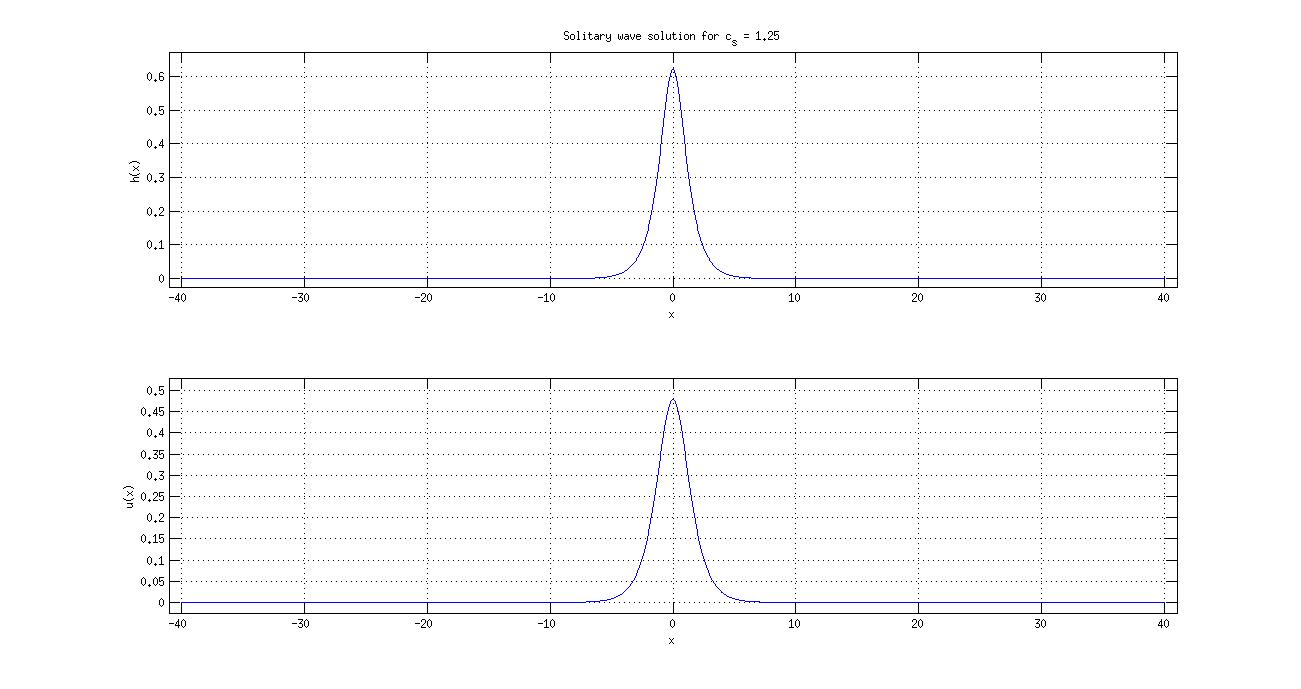
\includegraphics[height=8cm]{PeregrineSolitonSolution.jpg}
					\caption{Initial condition for the velocity and the free surface}
				\end{figure}
				
				For different time stepping methods and using or no different stabilization, we compute the solution and compare it to the initial condition at T=3.0s (during which the soliton moved of about 25 meters). 
				\begin{figure}[!h]
				\centering
						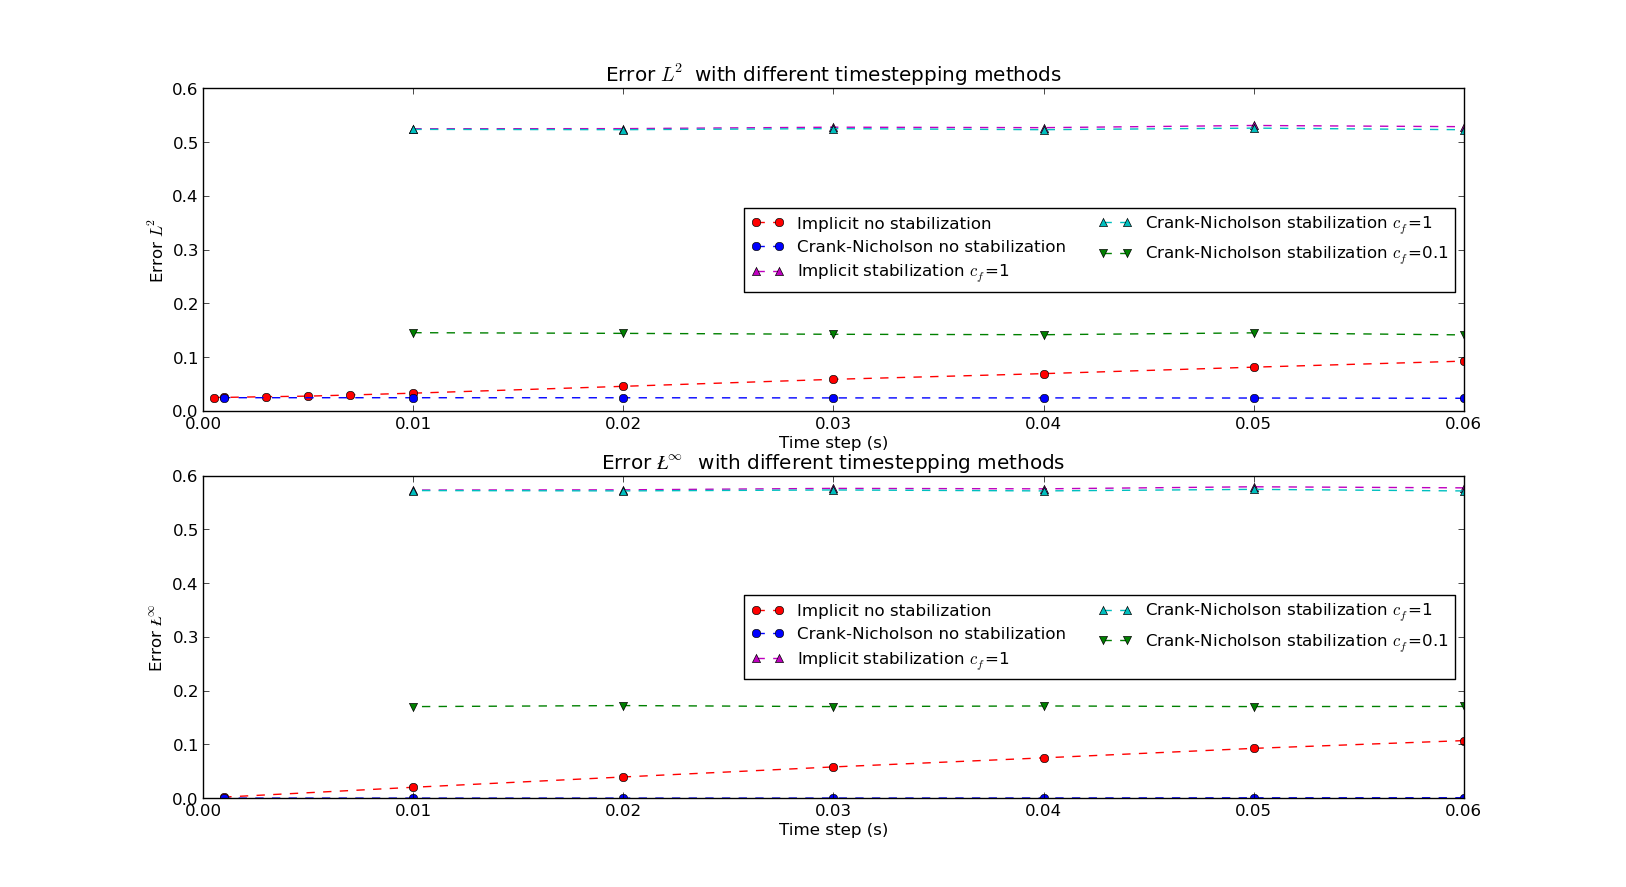
\includegraphics[height=9cm]{ErrorL2L801.png}
						\caption{Error}
				\end{figure}
	
		\subsection{Stabilization}
			\pagebreak
		\subsection{Time stepping methods}
			We tried two time-stepping methods in our weak formulation:
			\begin{itemize}
				\item Implicit method
				\item Crank-Nicholson schema
			\end{itemize}
			The implicit method is more stable than the Crank-Nicholson one, but add dissipation. We can see on the following figure the comparison of those two methods without stabilization and a stabilized simulation.
			\begin{figure}[!h]
				 \includegraphics[height=6.5cm]{ComparisonTimestepStabilization}
			\end{figure}
			
			\pagebreak				
	\section{Optimization}
		In this part we will focus on the optimization of the wave object so as to minimize a given functional characterizing the quality of the final water wave.
		A typical functional which will be used to assess the wave is the $H^1$ norm of the height of the free surface  $\eta$ at a final time $T$ over a specific domain $\omega$.
		\begin{equation}
			\inf_{\zeta_0 \in U_{ad}}\left\{J(\zeta_0)\ = \int_{\omega}{\! j(\eta(T),\zeta_0) \: \mathrm{dx}} \right\}, \: \mathrm{with} \: j(\eta(T),\zeta_0) = \frac{1}{2}||\eta(T)||_{H^1(\Omega)}^2
		\end{equation}
		\begin{figure}[!h]
			\centering
			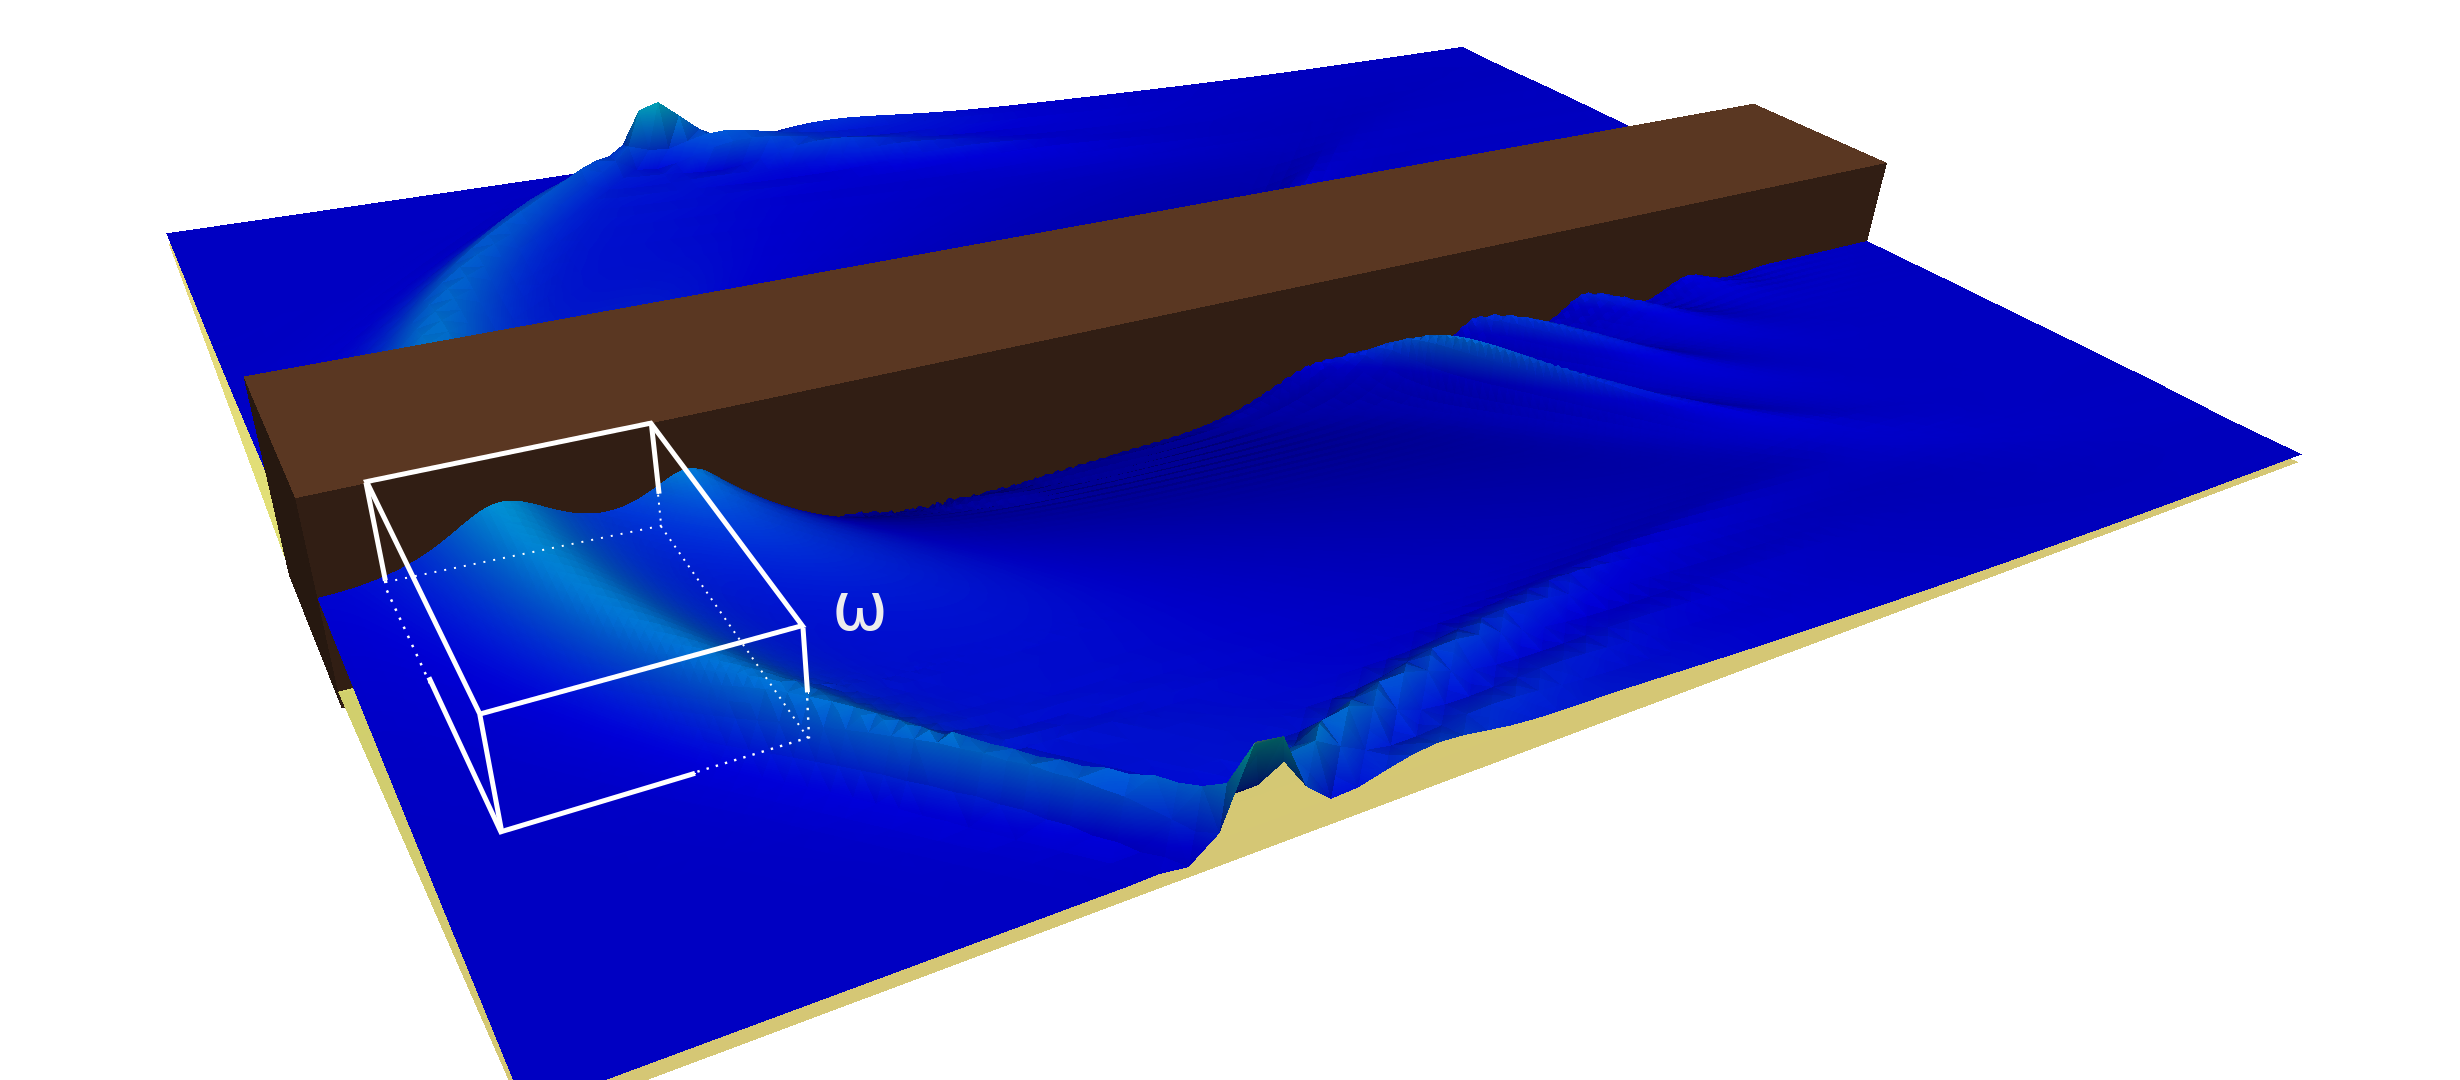
\includegraphics[height=5cm]{OptimizationDomain}
			\caption{Domain $\omega$ on which the wave is assessed}
		\end{figure}
		
		The set $U_{ad}$ of the admissible shape includes only object located at the central lane of the pool and with a determined maximal width and height.
		
		\begin{figure}[!h]
			\centering
			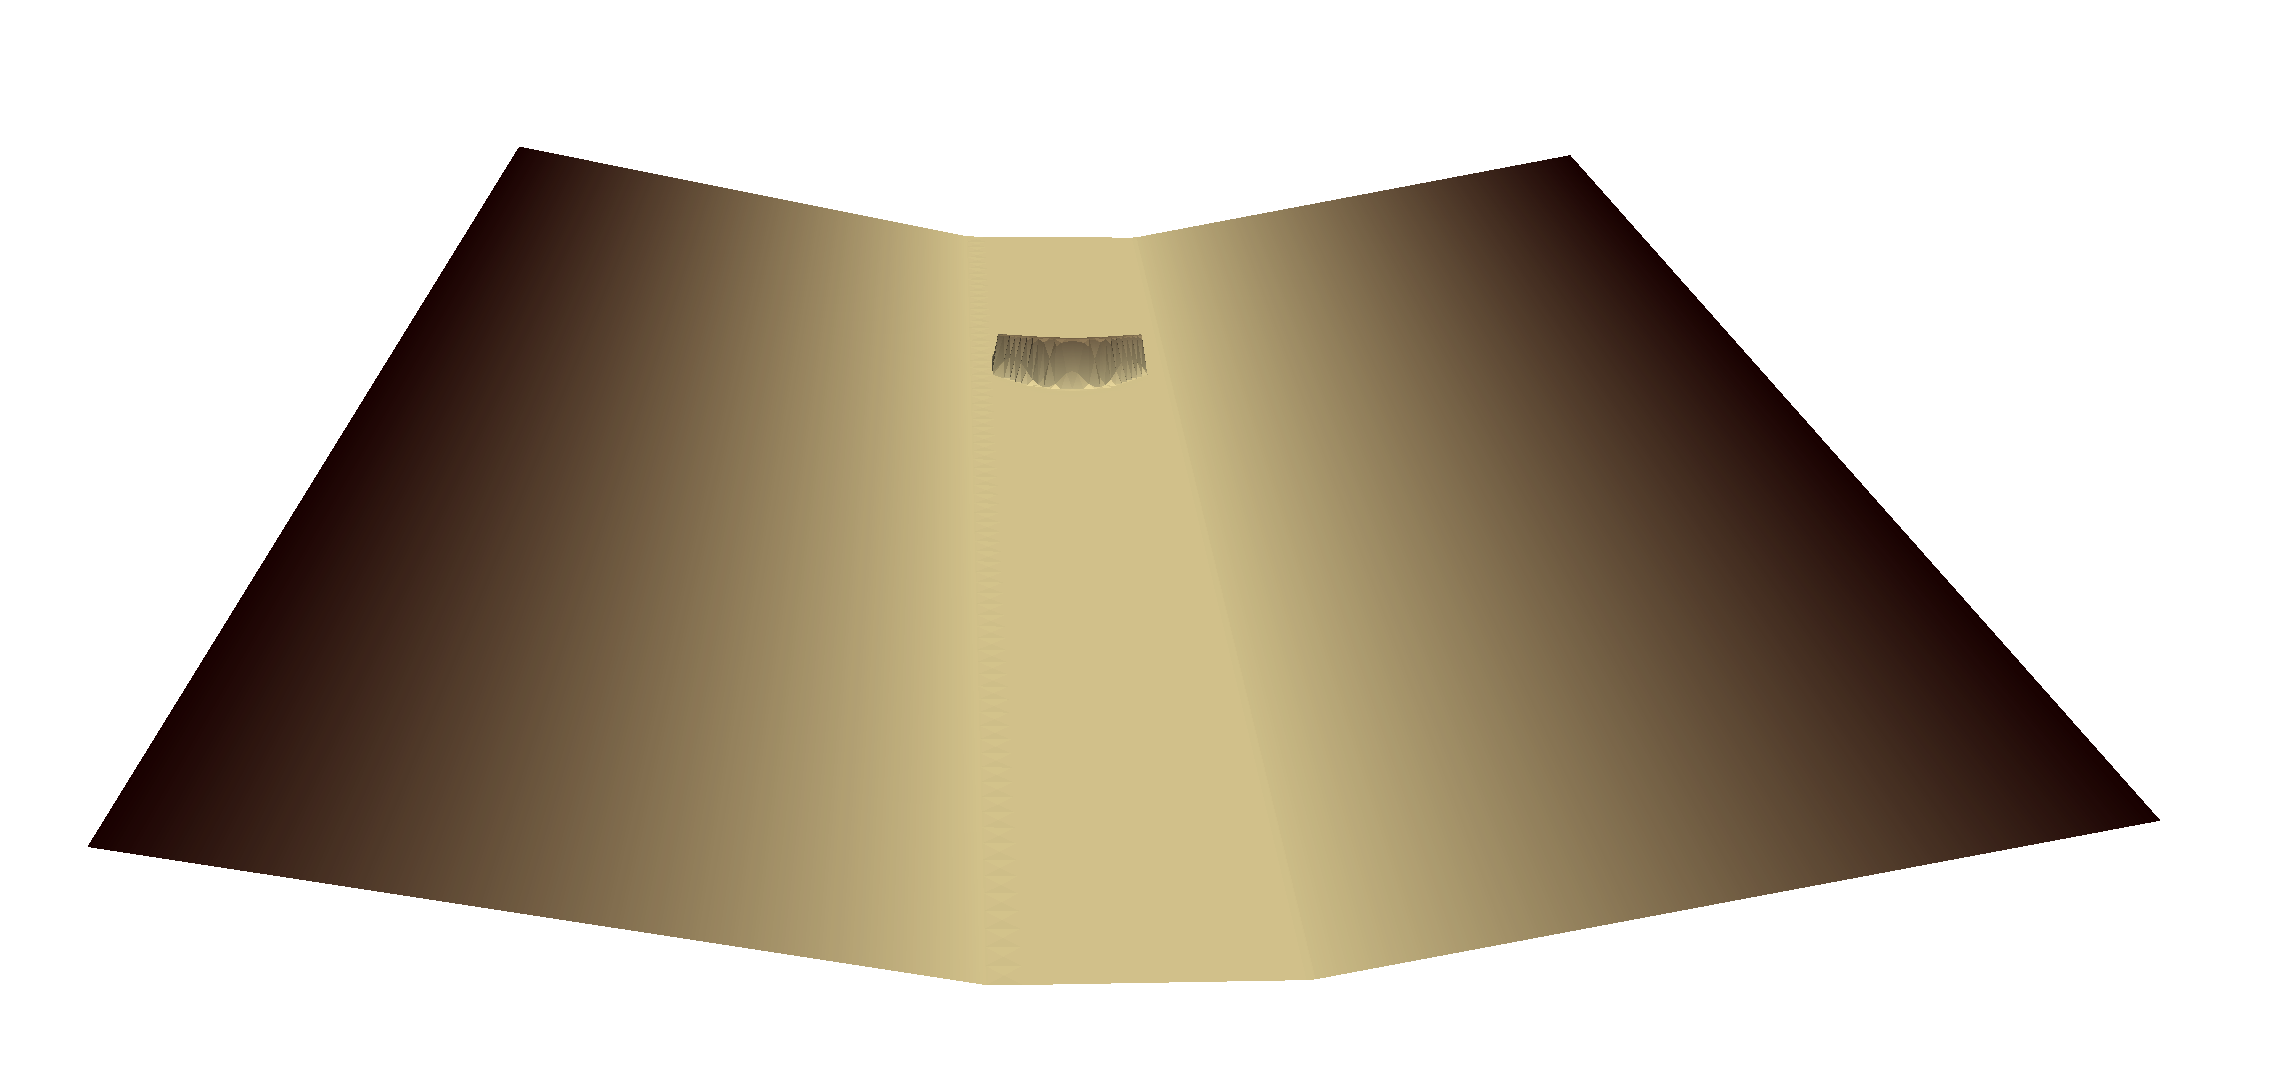
\includegraphics[height=5cm]{Object}
			\caption{Shape of the object}
		\end{figure}
				
		\subsection{Derivation of the adjoint system}
		Calling $(\mathbf{v}^N, \xi^N), ... (\mathbf{v}^0, \xi^0)$ the Lagrange multipliers associated with $(\mathbf{u}^N, \eta^N), ... (\mathbf{u}^0, \eta^0)$, we can now define the Lagrangian $\mathcal{L} $ of our problem: 
		
		\begin{align}
		\mathcal{L}(\zeta_0, (\mathbf{u}^N, \eta^N), ... (\mathbf{u}^0, \eta^0), 	(\mathbf{v}^N, \xi^N), ... (\mathbf{v}^0, \xi^0))	= J(\zeta_0) + \sum_{k=0}^{k=N-1} FV
		\end{align}
		
		\subsection{Coupling with the transport equation}
			We met some difficulties with FEniCS to optimize a time-dependent parameter. On the contrary, FEniCS and Dolfin Adjoint make it very easy to optimise parameters	such as an initial condition. A first approach to this optimization problem we shall consider is therefore the weakly coupled system below, in which the control is $\zeta_0(x,y)$.
		\begin{align}
			\mathbf{u}_t + \nabla \eta + \epsilon (\mathbf{u} \cdot \nabla)\mathbf{u} - \sigma^2\frac{h}{2}\nabla (\nabla \cdot (h \mathbf{u}_t)) + \sigma^2 \frac{h^2}{6}\nabla (\nabla \cdot \mathbf{u}_t) - \sigma^2\frac{h}{2}\nabla \zeta_{tt}  &= 0\\
			\eta_t+\zeta_t + \nabla \cdot [(h+\epsilon\eta)\mathbf{u}] &= 0 \\
			\zeta_t + \epsilon \mathbf{U} \cdot \nabla \zeta &= 0\\
			\zeta(x,y,t=0) &= \zeta_0(x,y)
		\end{align}
		where $\mathbf{U}(t)$ is the trajectory of the object.
				
				The main problem raised by this method is the instability of the transport equation, as we try to solve it with a finite element method. To be able to optimize correctly the shape of the object, we need however to transport this shape along the object trajectory with a good accuracy. The following part will present a few methods used to solve this equation. The lector is invited to see \cite{Transport} for more details on that topic.
				
					\subsubsection{Stabilization of the transport equation using Taylor-Galerkin method}
					A first method used to stabilize the transport equation, and which gives good results is a second-order Taylor-Galerkin approximation.
					Let $\Delta t$ be a small time-step and $\theta \in [0,1]$ the time-stepping method used, we have:	
					\begin{align}
						\displaystyle \frac{\zeta^{n+1} - \zeta^n}{\Delta t} = \left(\frac{\partial \zeta}{\partial t} \right)^n + \frac{\Delta t}{2} \left(\frac{\partial^2 \zeta}{\partial t^2} \right)^{n+\theta} + O(\Delta t^2)
					\end{align}
					using the transport equation
					\begin{equation}
						\displaystyle \frac{\partial \zeta}{\partial t} = - \epsilon \mathbf{U} \cdot \nabla \zeta, \qquad \displaystyle \frac{\partial^2 \zeta}{\partial t^2} = - \epsilon \frac{\partial \mathbf{U}}{\partial t} \cdot \nabla \zeta - \epsilon \mathbf{U} \cdot \nabla \frac{\partial \zeta}{\partial t}
					\end{equation}
					we get:
					\begin{align}
						\displaystyle \frac{\zeta^{n+1} - \zeta^n}{\Delta t} =- \epsilon \mathbf{U}^n \cdot \nabla \zeta^n - \frac{\epsilon \Delta t}{2} \left(\frac{\partial \mathbf{U}}{\partial t} \cdot \nabla \zeta^{n+\theta} - \epsilon \mathbf{U}^{n+\theta} \cdot \nabla (\mathbf{U}^{n+\theta} \cdot \nabla \zeta^{n+\theta})\right) + O(\Delta t^2)
					\end{align}
					which lead us to the following weak formulation: $\forall \tau \in \mathbb{H}^1_0(\Omega)$,
					\begin{align}
						\displaystyle \int_{\Omega}{\! \tau \frac{\zeta^{n+1} - \zeta^n}{\Delta t}}  -   \epsilon \int_{\Omega}{\! \nabla \tau \cdot  \mathbf{U}^n  \zeta^n} - \frac{\epsilon \Delta t}{2} \int_{\Omega}{\! \nabla \tau \cdot \frac{\partial \mathbf{U}}{\partial t} \zeta^{n+\theta}}
						 +  \frac{\epsilon^2 \Delta t}{2} \int_{\Omega}{\! (\nabla \tau \cdot \mathbf{U})(\nabla \zeta^{n+\theta} \cdot \mathbf{U}^{n+\theta})} = 0
					\end{align}
					Will the same method, a Taylor series expanded to the order 3 would give us the following:  $\forall \tau \in \mathbb{H}^1_0(\Omega)$,
					\begin{align*}
						& \displaystyle \int_{\Omega}{\! \tau \frac{\zeta^{n+1} - \zeta^n}{\Delta t}}  -   \epsilon \int_{\Omega}{\! \nabla \tau \cdot  \mathbf{U}^n  \zeta^n} + \frac{\Delta t}{2}\left( - \epsilon \int_{\Omega}{\! \nabla \tau \cdot \frac{\partial \mathbf{U}}{\partial t} \zeta^{n+\theta}}
						 +  \epsilon^2 \int_{\Omega}{\! (\nabla \tau \cdot \mathbf{U})(\nabla \zeta^{n+\theta} \cdot \mathbf{U}^{n+\theta})}\right) \\
						 & -\frac{\Delta t^2}{6}\left(\epsilon \int_{\Omega}{\! \nabla \tau \cdot \frac{\partial^2 \mathbf{U}}{\partial t^2} \zeta^{n+\theta}} -2*\epsilon^2 \int_{\Omega}{\! (\nabla \tau \cdot \frac{\partial \mathbf{U}}{\partial t})(\nabla \zeta^{n+\theta} \cdot \mathbf{U}^{n+\theta})} -\epsilon^2 \int_{\Omega}{\! (\nabla \zeta^{n+\theta} \cdot \frac{\partial \mathbf{U}}{\partial t})(\nabla \tau \cdot \mathbf{U}^{n+\theta})}\right) \\
						 & -\frac{\Delta t}{6} \epsilon^2 \int_{\Omega}{\! (\nabla \tau \cdot \mathbf{U})(\nabla (\zeta^{n+1} -  \zeta^n) \cdot \mathbf{U}^{n+\theta})}  = 0
					\end{align*}
					
					Comment the results of that method (the object do not keep is shape...)
					
				\subsection{Convergence}
					We use dolfin-adjoint coupled with pyipopt, which allows an automatic resolution of the adjoint system.
					
					
					
					
		
	
		\pagebreak	
	
	\section*{Annexes}
		\addcontentsline{toc}{section}{Annexe}
		
		\pagebreak
		
		\bibliographystyle{apalike} 
		\bibliography{Biblio}
		
		\appendix

\end{document}





